\subsection{Fit strategy and data selection}
\label{sec:fit_strategy}

All amplitudes in this section are for the isovector $u-d$ combination. The real unpolarized amplitude $\tAmp_{2B}^{\text{Re}}$ has small statistical errors over the whole lattice parameter space. The imaginary unpolarized amplitude $\tAmp_{2B}^{\text{Im}}$ and the real Sivers amplitude $\tAmp_{12B}^{\text{Re}}$ are noisier, and $\tAmp_{12B}^{\text{Im}}$ was dropped in Sec.~\ref{sec:amplitudes_lattice}. We parametrize the amplitudes in the Cartesian variables $(b_L,b_T,\eta)$, where $b_L=(P\cdot b)/(-P_L)$ and $b_T^2=b^2-b_L^2$. This uses all lattice points and separates the longitudinal from the transverse profile, which the compressed variables $(P\cdot b,b^2)$ do not.

\paragraph{Gaussian profile.}
A 2D Gaussian, $\tAmp^{\text{Re}}_{iB}=\gamma\exp[-\alpha b_L^2-\beta b_T^2]$, becomes $\gamma\exp[-\tfrac{\alpha-\beta}{P_L^2}(P\cdot b)^2-\beta b^2]$ in the invariant variables. The Fourier integral over $P\cdot b$ converges only for $\alpha>\beta$. The fit to $\tAmp^{\text{Re}}_{2B}$ gives $\alpha-\beta=-0.0427(27)$ with $\chi^2/\text{dof}\approx 235$ at $P_L=-1$ (Fig.~\ref{fig:gaussian_fail}), so the Gaussian is both a poor description and not Fourier-integrable.

\paragraph{Short-distance cut.}
At $|\vect{b}|\sim a$ or $2a$ the operator is affected by hypercubic-symmetry breaking, $\mathcal O(a)$ and $\mathcal O(a^2)$ link-path artifacts, and incipient short-distance divergences, while we want the medium-range nonperturbative behavior. We therefore keep only $|\vect{b}|\ge 3a$. Fig.~\ref{fig:short_distance} shows the difference in the data: at fixed $b^2$, the short-distance amplitude rises with $|P\cdot b|$ by about $14\%$ for $b^2/a^2=5$, while it stays flat within errors for $b^2/a^2=20$ and $45$.

\paragraph{Staple extent.}
The Sivers shift requires $\eta\to\infty$. The first-moment study of Ref.~\cite{Musch:2011er} found that the shift reaches a plateau for $|\eta v|=7a\ldots12a$, which indicates that the Sivers and unpolarized TMDs share a common $\eta$ profile that cancels in the ratio. We therefore perform global fits in $(b_L,b_T,\eta)$ over $6\le\eta\le10$.

\begin{figure}
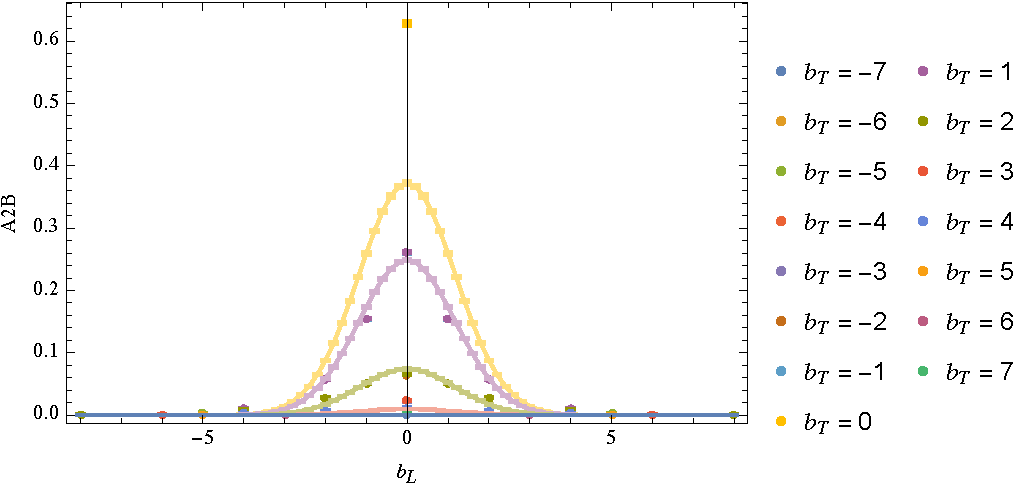
\includegraphics[width=\columnwidth]{figures/results/gaussian_fail_A2B.pdf}
\caption{Failure of the Gaussian model for $\tAmp_{2B}^{\text{Re}}$ at $P_L=-1$ ($\alpha-\beta=-0.0427(27)$, $\chi^2/\text{dof}\approx235$).}
\label{fig:gaussian_fail}
\end{figure}

\begin{figure}
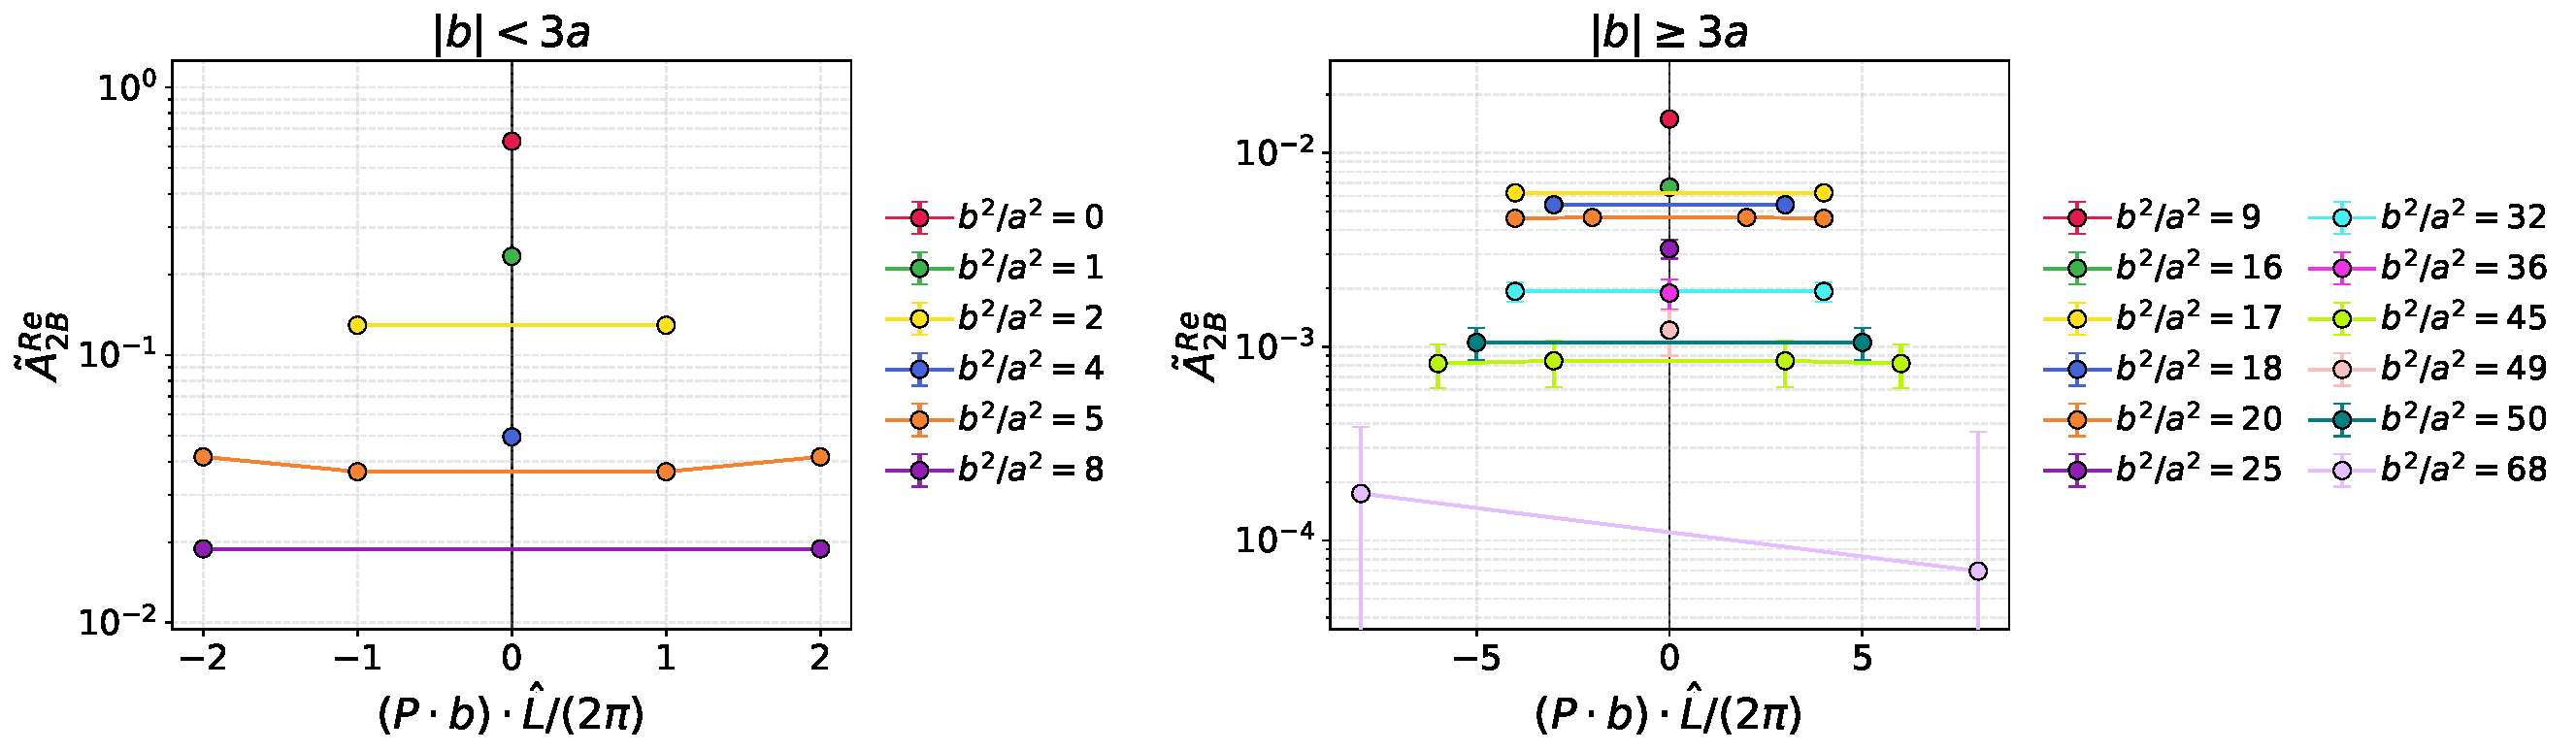
\includegraphics[width=\columnwidth]{figures/results/short_distance.pdf}
\caption{$\tAmp_{2B}^{\text{Re}}$ at $P_L=-1$ and $\eta|\vect v|/a=9$ for $|\vect b|<3a$ (left) and $|\vect b|\ge3a$ (right). Points with equal $b^2$ are connected to guide the eye.}
\label{fig:short_distance}
\end{figure}

\subsection{Global power-law fit}
\label{sec:global_fit}

Symbolic regression with \texttt{PySR}~\cite{Cranmer2023pysr}, using a custom loss that penalizes growth at large $b_L$, points to a power-law tail $(1+b^2)^{-j}$ multiplied by an exponential $e^{-f\eta}$ and never selects a Gaussian profile (Appendix~\ref{app:fit_exploration}). We then explored the $\eta$ dependence of the power-law model, and compared it with exponential and other separable longitudinal-transverse forms (Appendix~\ref{app:fit_exploration}). The separable forms either have a longitudinal coefficient consistent with zero, so that the Fourier transform to $x$ does not exist, or fail for $\tAmp_{2B}^{\text{Im}}$ and $\tAmp_{12B}^{\text{Re}}$. The selected models are
\begin{align}
\tAmp_{2B}^{\text{Re}}&=\frac{a\,e^{-f\eta}}{\big[1+\big(d+c\,(1-\tfrac{k_1}{\eta}-\tfrac{k_2}{\eta^2})\big)b_L^2+d\,b_T^2\big]^{j}}\,,\label{eq:model_ReA2B}\\
\tAmp_{2B}^{\text{Im}}&=\frac{a''\,b_L\,e^{-f\eta}}{\big[1+(c''+d'')b_L^2+d''b_T^2\big]^{j''}}\,,\label{eq:model_ImA2B}\\
\tAmp_{12B}^{\text{Re}}&=\frac{-a'\,e^{-f\eta}}{\big[1+(c'+d')b_L^2+d'b_T^2\big]^{j'}}\,.\label{eq:model_ReA12B}
\end{align}
The $\eta$ dependence of $c$ in $\tAmp_{2B}^{\text{Re}}$ was chosen among several candidates with equal $\chi^2/\text{dof}$ by requiring that the antiquark region $x\lesssim-0.2$ of $\tilde f_1^{(0)}$ is suppressed at large momentum and that the $x$-integrated results agree with earlier first-moment calculations~\cite{Musch:2011er,Yoon:2017qzo}. For $\tAmp_{12B}^{\text{Re}}$, the slopes of $c$ and $d$ against $\eta$ are consistent with zero within about $1\sigma$, and for $d$ of $\tAmp_{2B}^{\text{Re}}$ the slope is $0.00122(87)$. For $\tAmp_{2B}^{\text{Im}}$ the slope of $d$ is within $1.5\sigma$ of zero and that of $c$ is about $2\sigma$ from zero. We keep these parameters constant in $\eta$ to avoid overfitting.

Since $e^{-f\eta}$ does not depend on $P\cdot b$, it cancels between numerator and denominator of the Sivers shift, Eq.~\eqref{eq:sivers_shift_xdep}, when it is shared by the three amplitudes. We therefore fit the three amplitudes simultaneously at each momentum with one common $f$, minimizing the correlated $\chi^2$ with the full Jackknife covariance matrix~\cite{Boram2011Covariance}, which includes correlations between different $(b_L,b_T,\eta)$ points and between the three amplitudes. The fits use \texttt{lsqfit}~\cite{Lepage:2001ym}. The global $\chi^2/\text{dof}$ is $1.85(10)$, $1.197(85)$, $0.712(66)$ and $0.434(51)$ for $P_L=-1,\ldots,-4$, and the fitted parameters are listed in Table~\ref{tab:fit_params} of Appendix~\ref{app:fit_exploration}. Fig.~\ref{fig:fit_example} compares the fit with the data for $P_L=-4$ at $\eta|\vect v|/a=8$.

\begin{figure*}
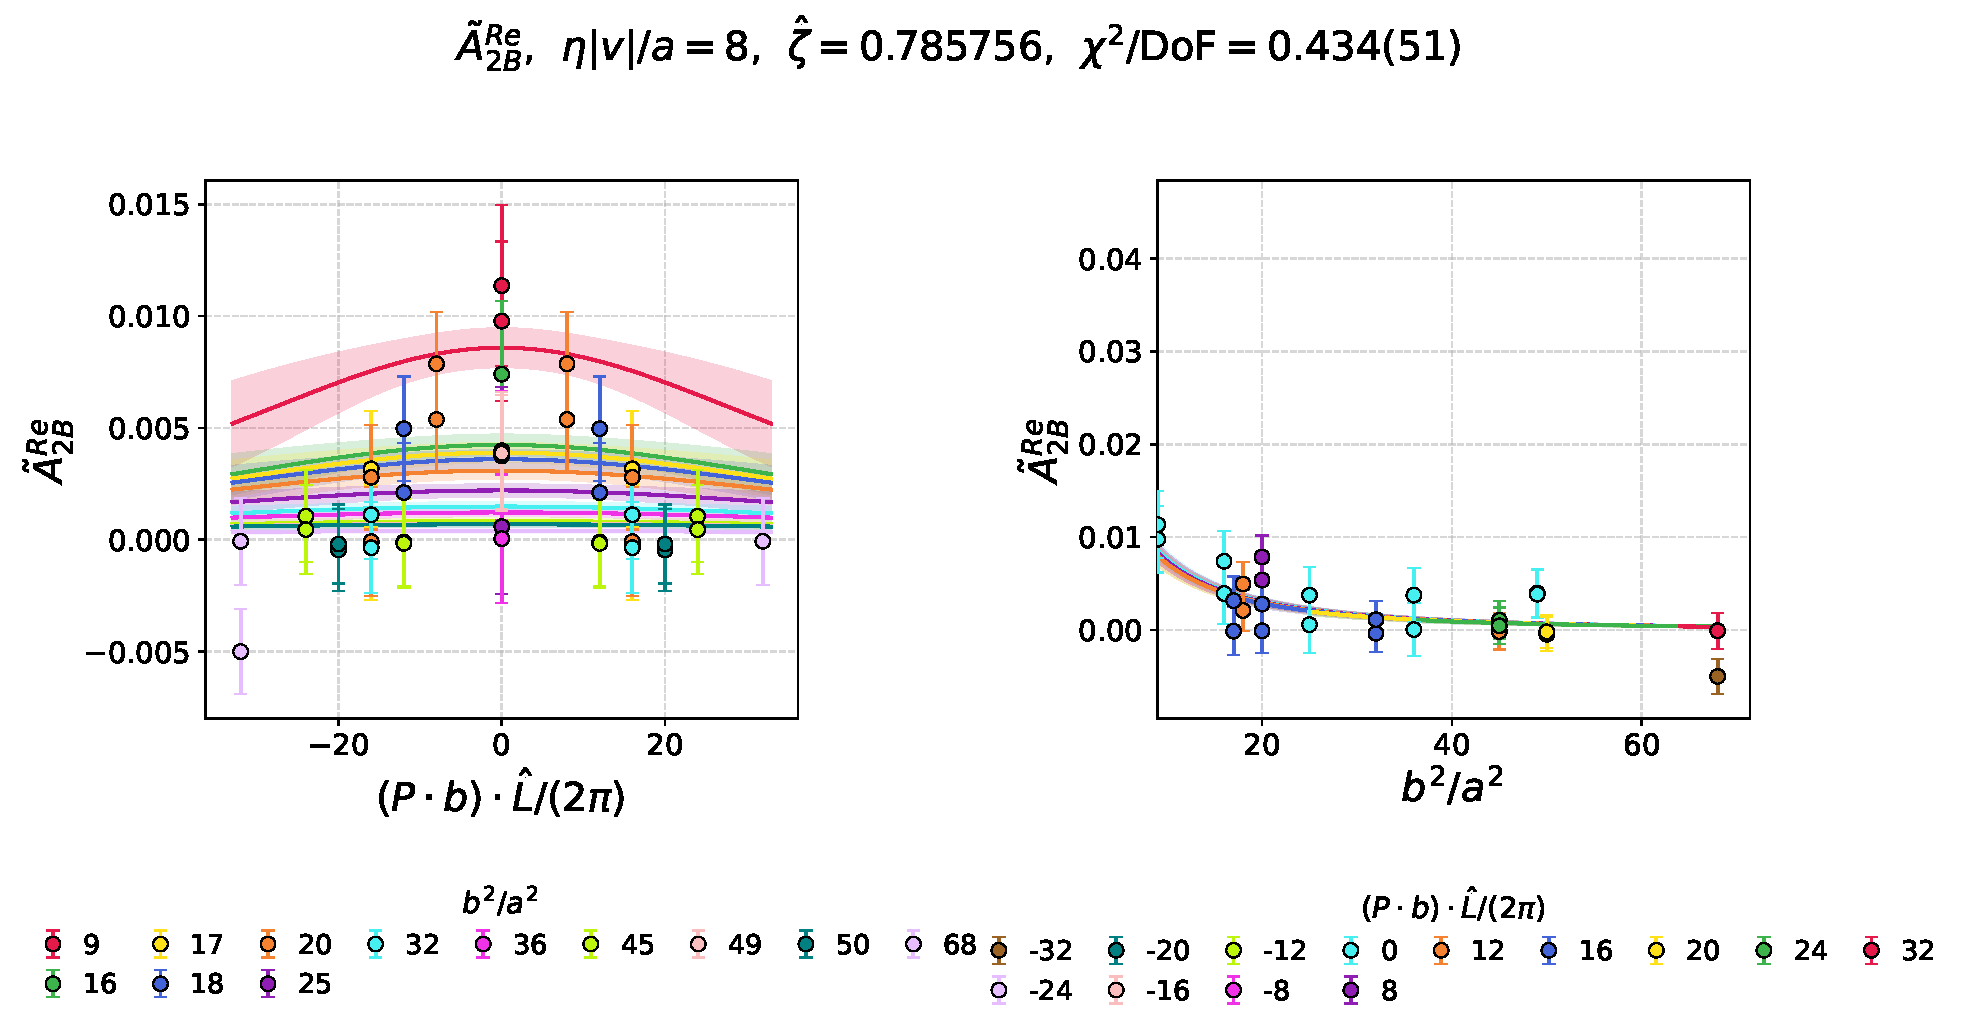
\includegraphics[width=0.32\textwidth]{figures/results/fit_ReA2B_PL-4_eta8.pdf}\hfill
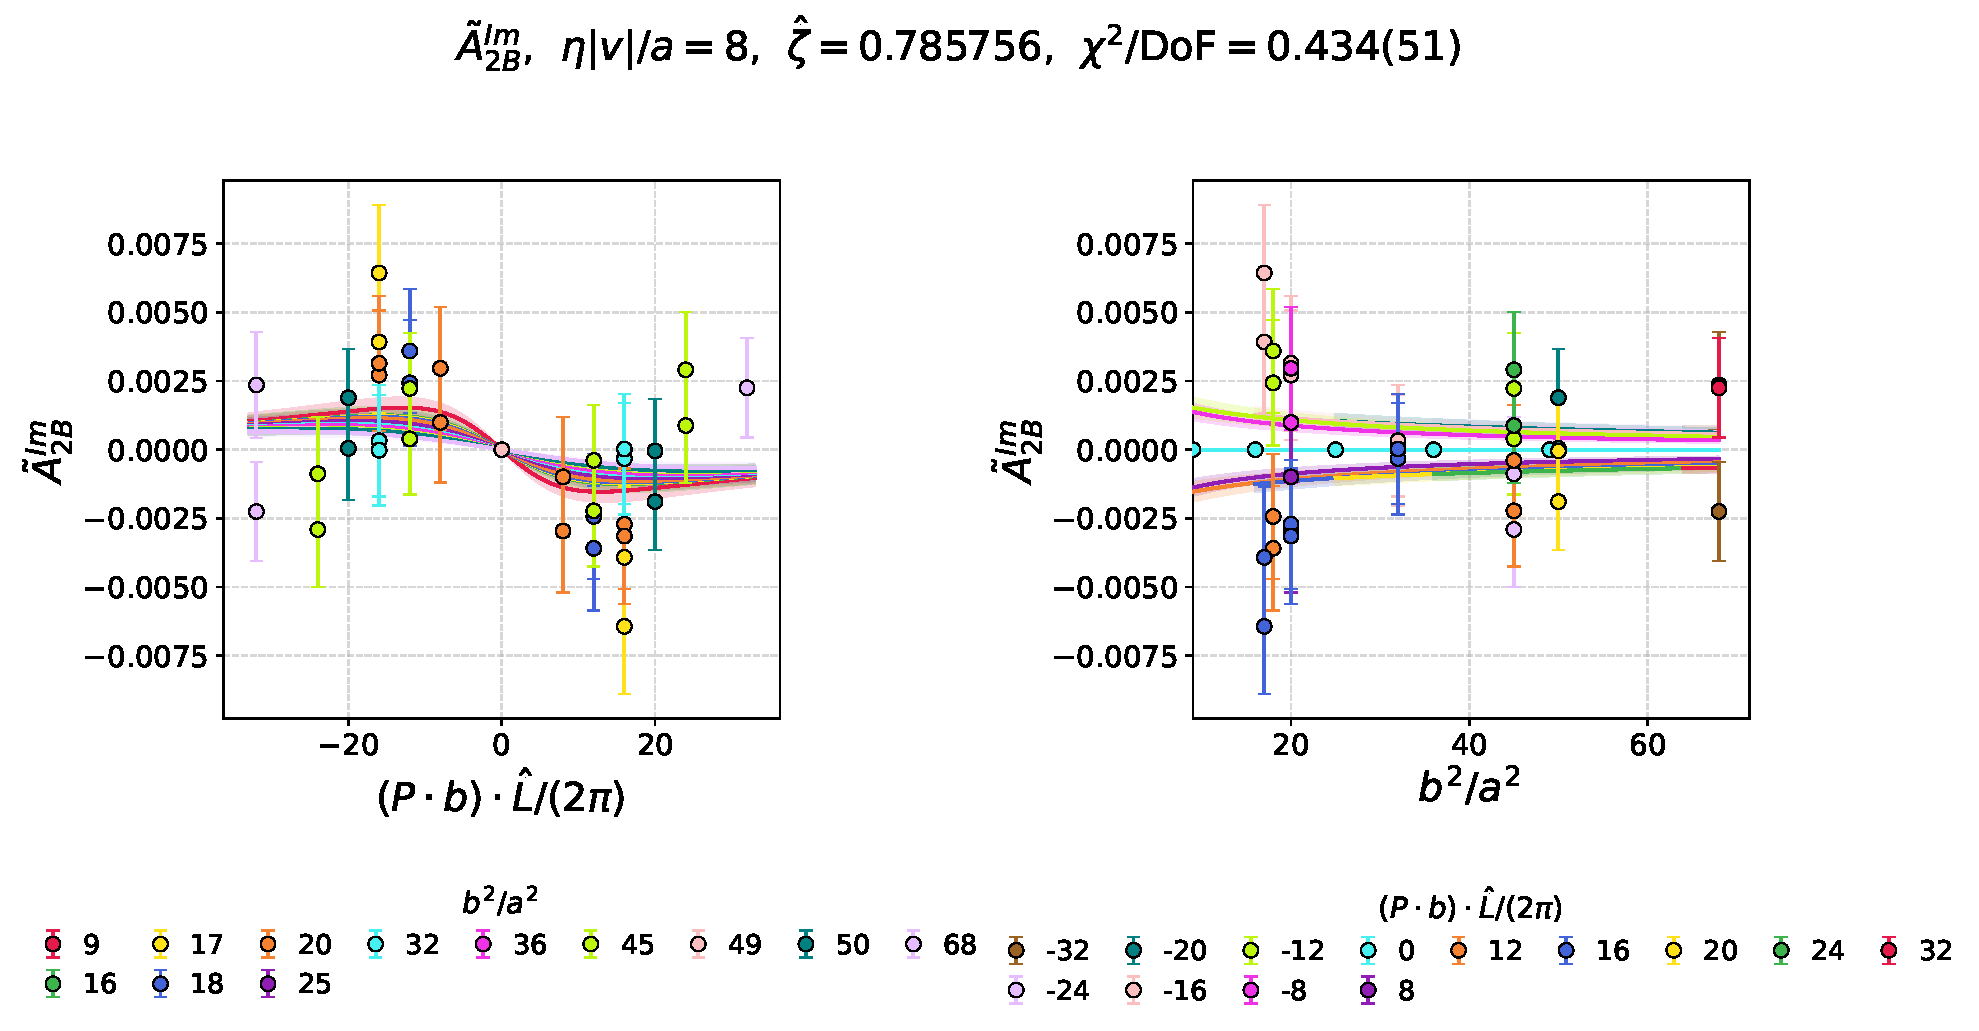
\includegraphics[width=0.32\textwidth]{figures/results/fit_ImA2B_PL-4_eta8.pdf}\hfill
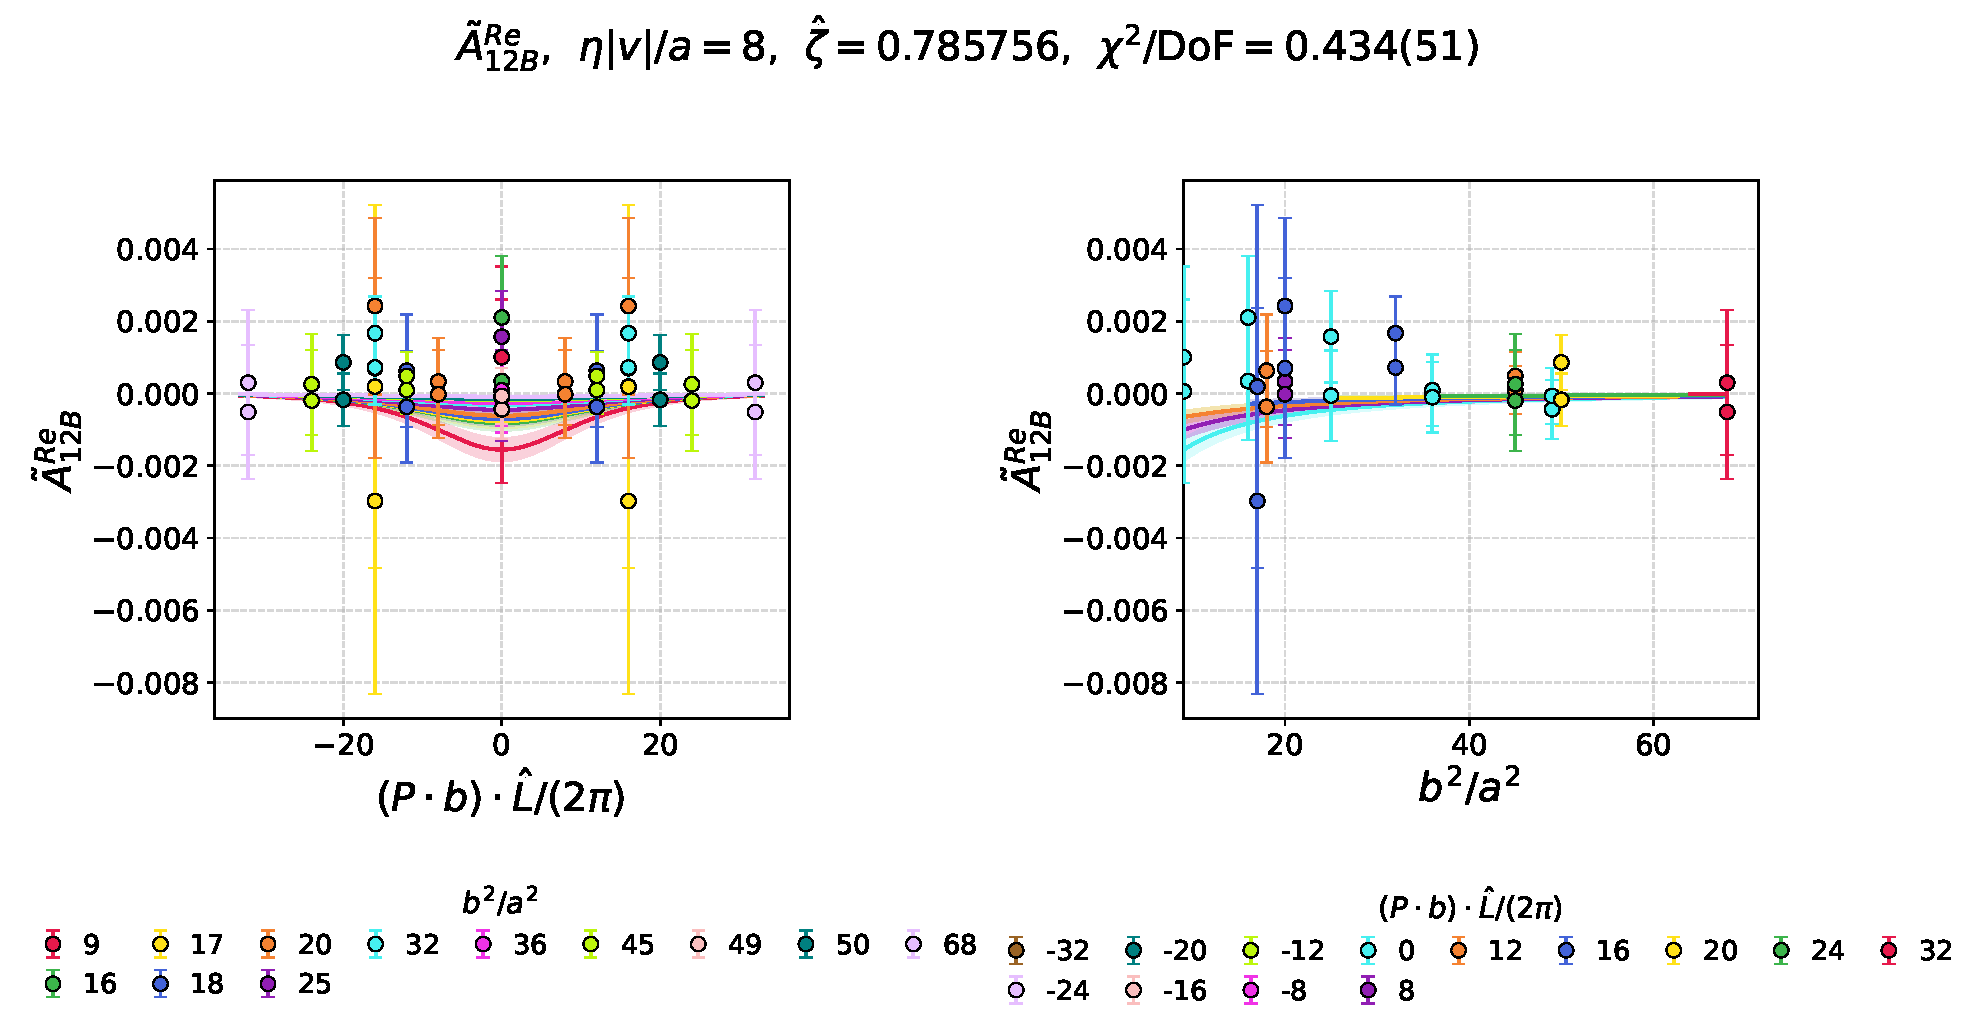
\includegraphics[width=0.32\textwidth]{figures/results/fit_ReA12B_PL-4_eta8.pdf}
\caption{Simultaneous fit for $P_L=-4$ at $\eta|\vect v|/a=8$ in the variables $(P\cdot b,b^2)$: $\tAmp_{2B}^{\text{Re}}$, $\tAmp_{2B}^{\text{Im}}$ and $\tAmp_{12B}^{\text{Re}}$ (left to right).}
\label{fig:fit_example}
\end{figure*}

\subsection{Extrapolation to $\hat\zeta\to\infty$}
\label{sec:zeta_extrapolation}

The simulated momenta $P_L=-1,\ldots,-4$ correspond to $\hat\zeta=0.090772$, $0.294367$, $0.539684$, $0.785756$, far from the $\hat\zeta\gg1$ regime relevant for comparison with factorization-based phenomenology. At fixed $|\vect b_T|=3a\approx0.34$~fm, the reconstructed amplitudes, the TMD combinations $\tilde f_1^{(0)}=2\tAmp_{2B}^{[x]}$ and $\tilde f_{1T}^{\perp(1)}=-2\tAmp_{12B}^{[x]\text{Re}}$, and the Sivers shift all vary systematically with $1/\hat\zeta$. Perturbative TMD evolution~\cite{Aybat:2011zv} suggests that ratios of TMDs become independent of $\hat\zeta$ as $\hat\zeta\to\infty$, which is the physical limit for the Sivers shift, where the soft factor cancels.

We extrapolate the fit parameters themselves rather than the amplitudes point by point in $x$. We exclude $P_L=-1$ ($1/\hat\zeta=11.02$), which lies far from the other three ($1/\hat\zeta=3.40$, $1.85$, $1.27$) and would dominate the extrapolated intercept. The parameters $c$ of the three amplitudes are first rescaled by $1/P_L^2$, and the parameter of the odd amplitude $\tAmp_{2B}^{\text{Im}}$ multiplying $b_L$ by $1/P_L$, so that they multiply powers of the invariant $P\cdot b$ at all momenta. We tested
\begin{equation}
p(\hat\zeta)=c_p+\frac{d_p}{\hat\zeta}\quad\text{and}\quad p(\hat\zeta)=c_p+\frac{d_p}{\hat\zeta^{2}}
\label{eq:zeta_ansatz}
\end{equation}
as in Ref.~\cite{Musch:2011er} with correlated Jackknife fits to the three momenta. The quadratic form gives a lower $\chi^2/\text{dof}$ for the parameters and we adopt it throughout (Fig.~\ref{fig:param_extrap}). The extrapolated value of each parameter is the intercept $c_p$. With only three momenta and two parameters per fit, this extrapolation has one degree of freedom and its systematic uncertainty is not captured by the Jackknife errors.

Reconstructing the amplitudes from the extrapolated parameters gives $\tilde f_1^{(0)}$, $\tilde f_{1T}^{\perp(1)}$ and the Sivers shift at $\hat\zeta\to\infty$ (Fig.~\ref{fig:extrap_sivers}). At $|\vect b_T|=0.34$~fm, $\langle k_y\rangle_{TU}$ peaks at about $0.21$~GeV at small $x$ and falls to near zero by $x\approx0.5$, while $x\langle k_y\rangle_{TU}$ peaks at about $0.02$~GeV near $x\approx0.15$. The overall sign reverses between the SIDIS and DY limits and the magnitude is unchanged. The extrapolated curve differs from all three finite-momentum curves that enter it, including the one at $P_L=-4$, so the extrapolation captures momentum dependence beyond the largest simulated momentum. Fig.~\ref{fig:extrap_sivers_3D} shows the dependence on $|\vect b_T|$ between $3a\approx0.34$~fm and $\sqrt{68}\,a\approx0.94$~fm.

Table~\ref{tab:integrals} lists the $x$-integrals of the extrapolated amplitudes at $|\vect b_T|=3a$. Integrating over $[-\infty,\infty]$ and $[-1,1]$ gives the same results within errors, so the truncation at $|x|=1$ is negligible. The imaginary term $\int dx\,\tAmp^{[x]\text{Im}}_{2B}$ vanishes over the symmetric ranges and has opposite sign for the quark and antiquark ranges, as required by its odd parity. The first four rows are unrenormalized and the multiplicative renormalization cancels only in the ratio in the last row.

\begin{table*}
\caption{$x$-integrals of the extrapolated ($\hat\zeta\to\infty$) amplitudes at $|\vect b_T|=3a\approx0.34$~fm for four integration ranges. The first four rows are unrenormalized.}
\label{tab:integrals}
\begin{ruledtabular}
\begin{tabular}{lcccc}
Integral & $[-\infty,\infty]$ & $[-1,1]$ & $[-1,0]$ & $[0,1]$ \\
\hline
$\int\!dx\,\tAmp^{[x]\text{Re}}_{2B}$ & $0.751(79)$ & $0.751(80)$ & $0.375(40)$ & $0.375(40)$ \\
$\int\!dx\,\tAmp^{[x]\text{Im}}_{2B}$ & $6(96)\!\times\!10^{-17}$ & $3(24)\!\times\!10^{-16}$ & $0.165(27)$ & $-0.169(29)$ \\
$\int\!dx\,\tilde f_1^{(0)}$ & $1.50(16)$ & $1.50(16)$ & $0.421(81)$ & $1.09(11)$ \\
$\int\!dx\,\tilde f_{1T}^{\perp(1)}$ & $0.302(53)$ & $0.302(53)$ & $0.151(27)$ & $0.151(27)$ \\
$\langle k_y\rangle_{TU}$ (GeV) & $0.217(38)$ & $0.217(38)$ & $0.387(89)$ & $0.150(26)$ \\
\end{tabular}
\end{ruledtabular}
\end{table*}

\begin{figure*}
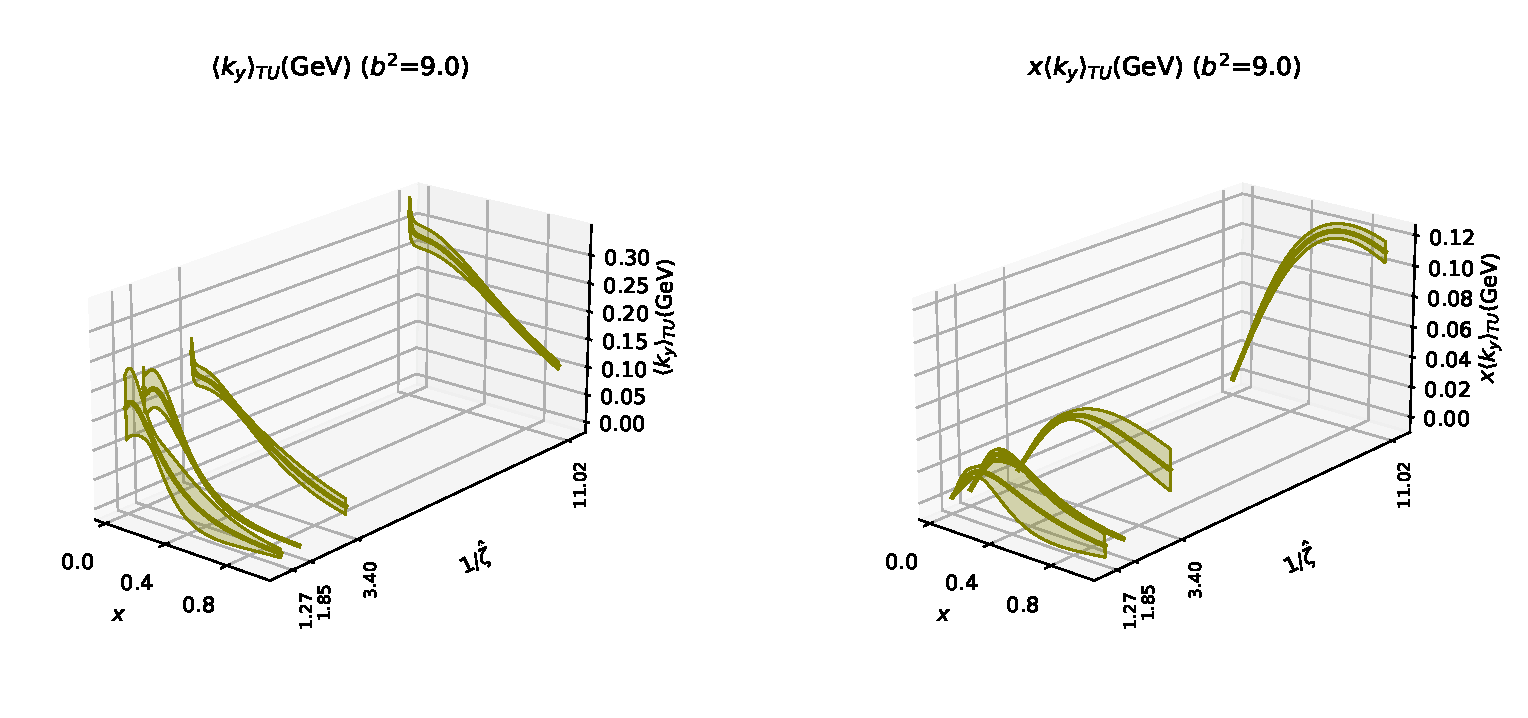
\includegraphics[width=0.9\textwidth]{figures/results/zetahat_slices_sivers.pdf}
\caption{Sivers shift $\langle k_y\rangle_{TU}$ and $x\langle k_y\rangle_{TU}$ at $|\vect b_T|=3a\approx0.34$~fm for the four simulated momenta, against $x$ and $1/\hat\zeta$ ($x\ge0$).}
\label{fig:zetahat_slices}
\end{figure*}

\begin{figure*}
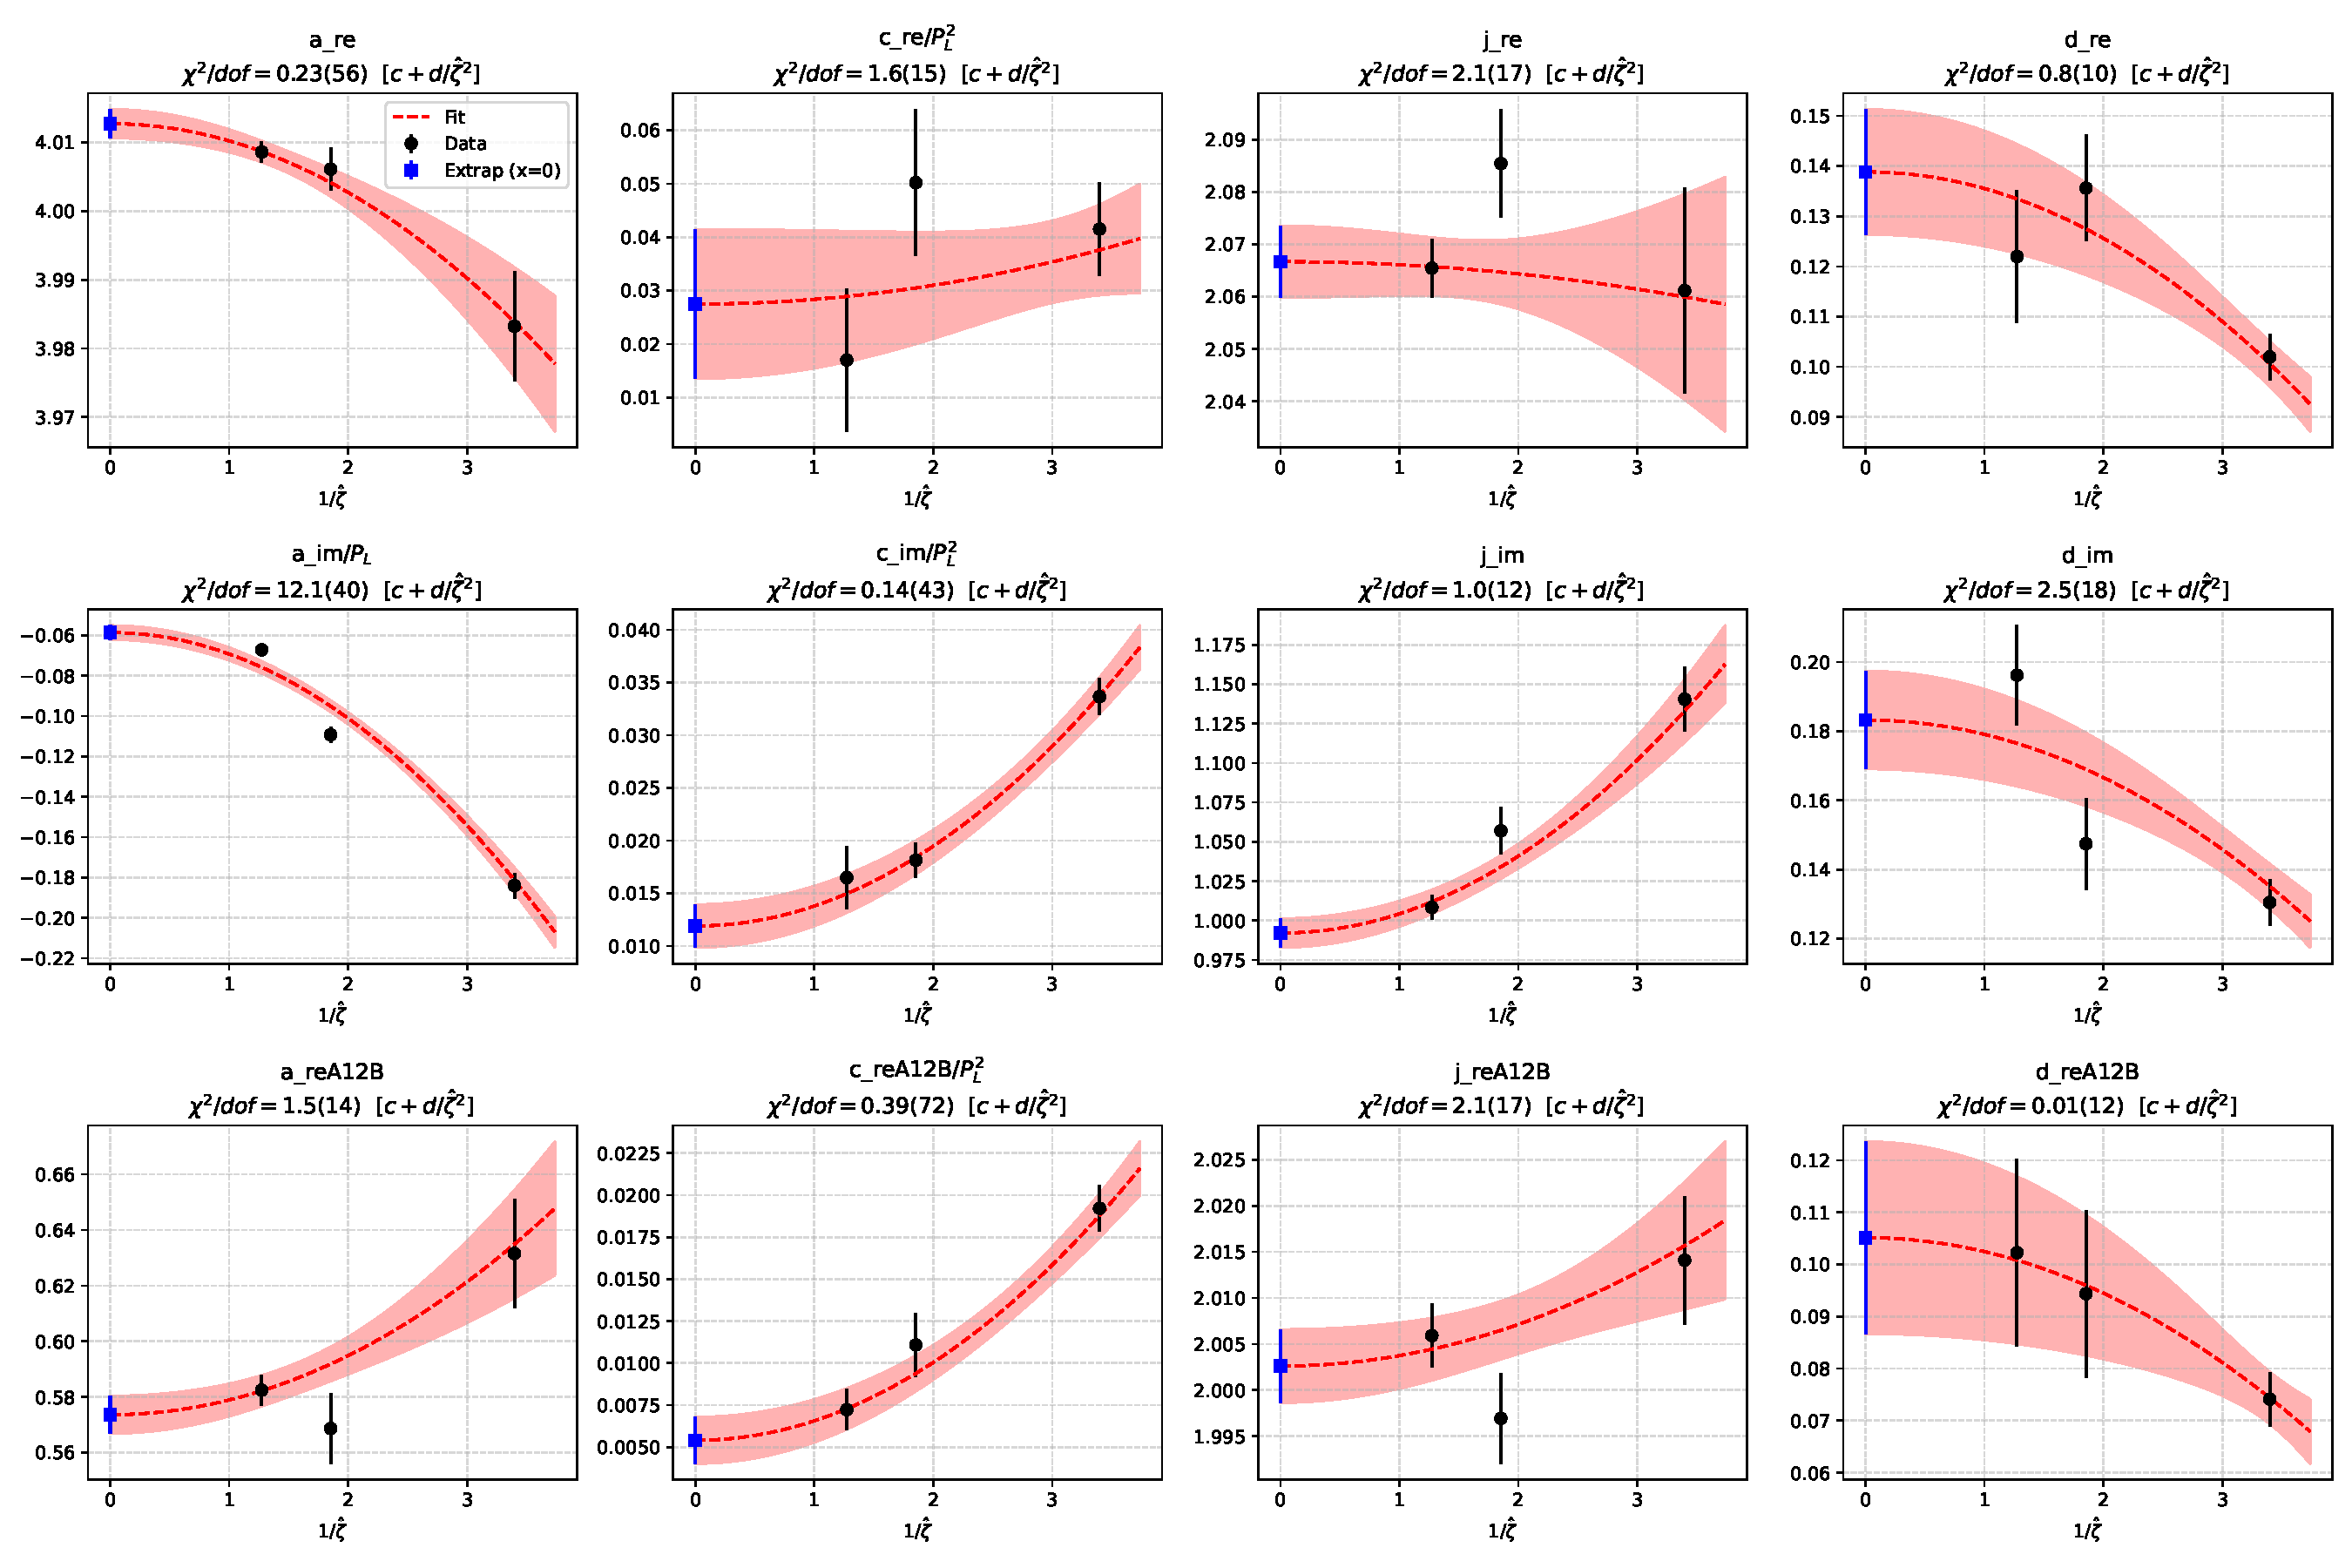
\includegraphics[width=0.75\textwidth]{figures/results/param_extrapolation.pdf}
\caption{Extrapolation of the twelve fit parameters to $\hat\zeta\to\infty$ using $P_L=-2,-3,-4$ (black), with the ansatz $c_p+d_p/\hat\zeta^2$ (red dashed, band) and the extrapolated value (blue square). Each panel title gives the Jackknife $\chi^2/\text{dof}$. The parameters $c$ are shown rescaled by $1/P_L^2$ and the coefficient of $b_L$ in $\tAmp_{2B}^{\text{Im}}$ by $1/P_L$.}
\label{fig:param_extrap}
\end{figure*}

\begin{figure*}
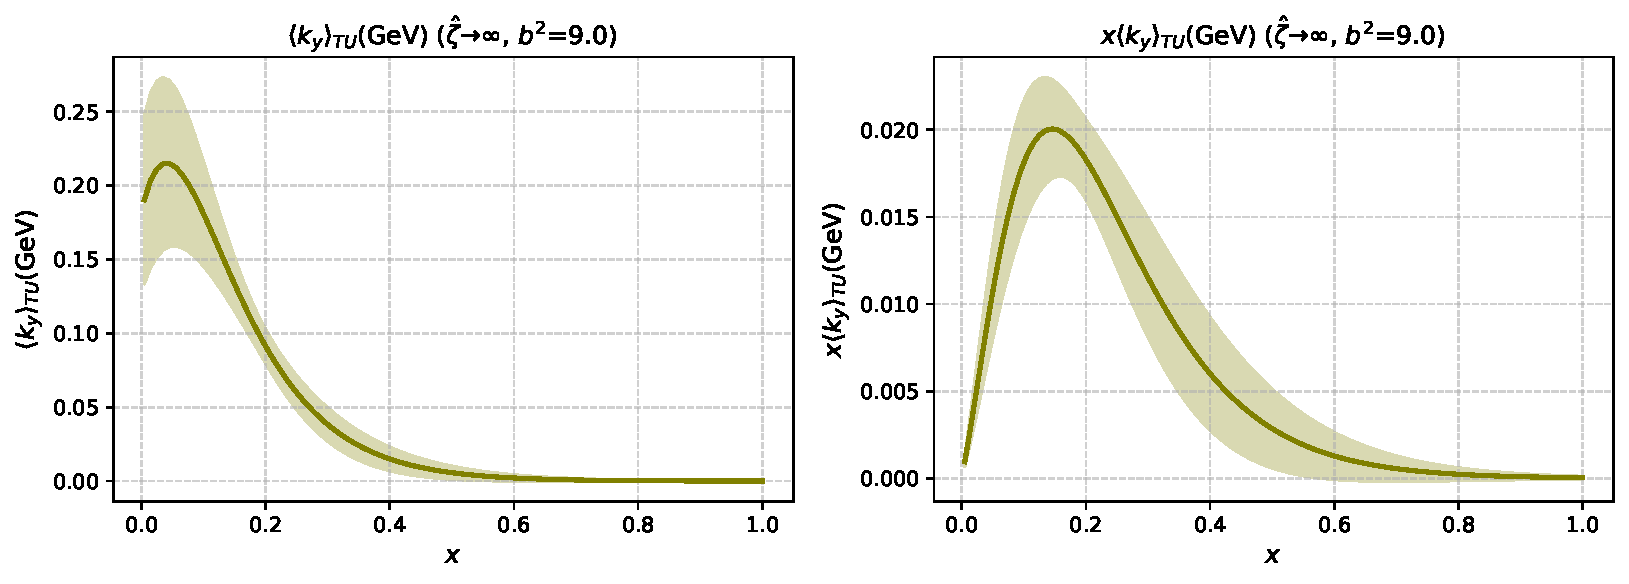
\includegraphics[width=0.9\textwidth]{figures/results/extrap_sivers.pdf}
\caption{Isovector Sivers shift $\langle k_y\rangle_{TU}$ and $x\langle k_y\rangle_{TU}$ at $\hat\zeta\to\infty$ for $|\vect b_T|=3a\approx0.34$~fm. Bands are Jackknife uncertainties propagated from the extrapolated parameters.}
\label{fig:extrap_sivers}
\end{figure*}

\begin{figure}
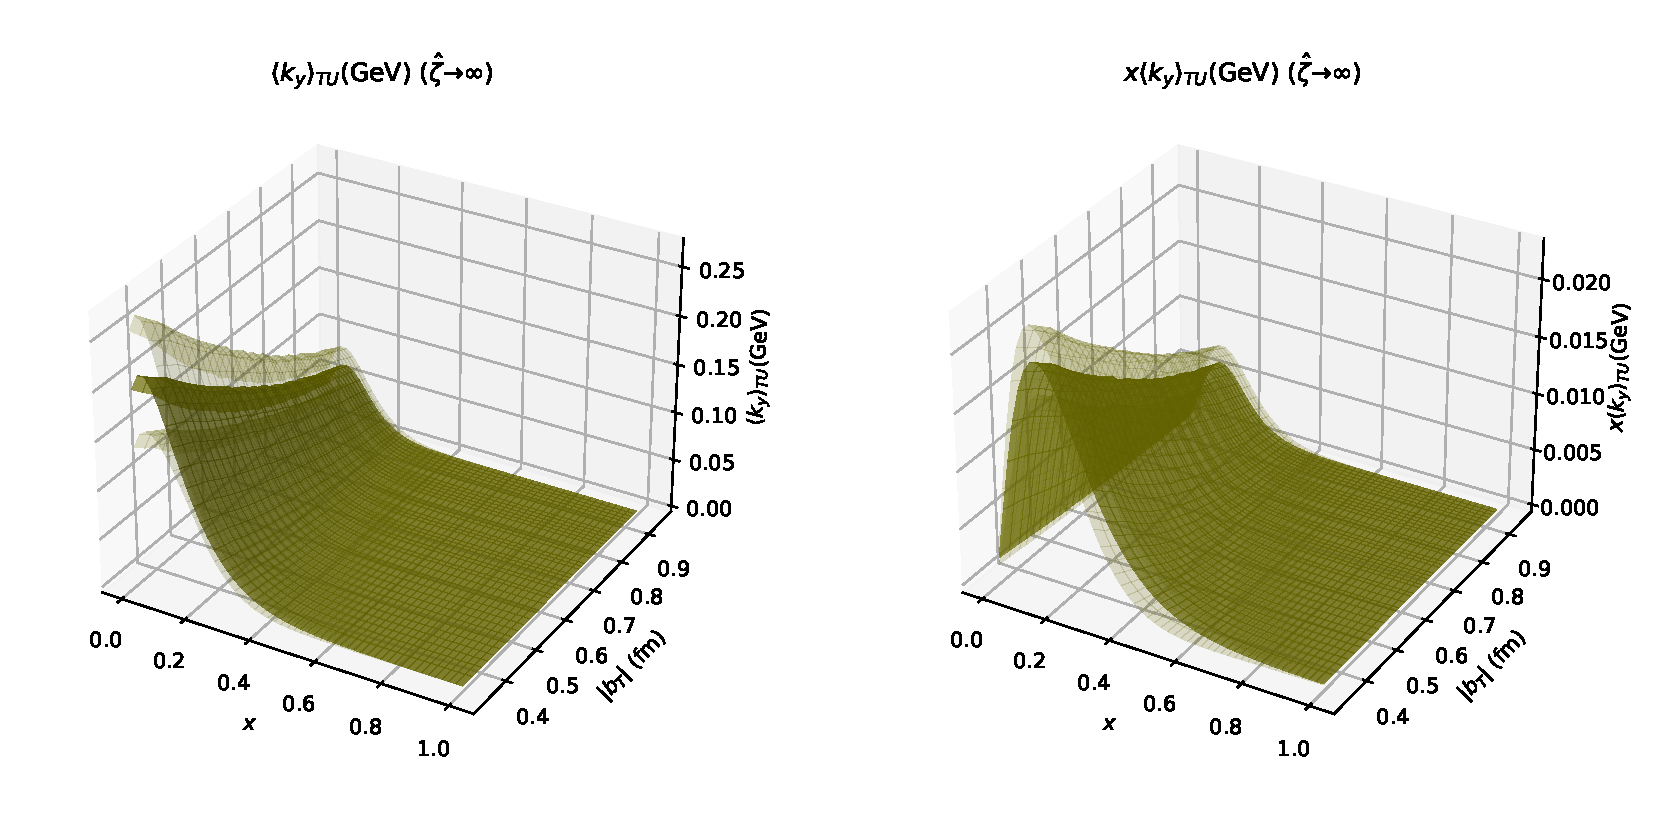
\includegraphics[width=\columnwidth]{figures/results/extrap_sivers_3D.pdf}
\caption{Extrapolated Sivers shift as a function of $x\ge0$ and $|\vect b_T|$ from $0.34$ to $0.94$~fm.}
\label{fig:extrap_sivers_3D}
\end{figure}

\subsection{Factorization in $x$ and $|\vect b_T|$}
\label{sec:factorization}

The global fit couples $(P\cdot b)$ and $b^2$, and the selected models are not products of separate functions of the two variables. The question is how far a factorized description, common in phenomenology, can nonetheless approximate the result. A recent symbolic-regression extraction of the unpolarized TMD from Drell-Yan data finds a mild but genuine $x$-$b_T$ correlation rather than strict separability~\cite{Granger:2026symb}.

\paragraph{Lattice data.}
We first test the data at finite momentum for the form $\tAmp(P\cdot b,b^2)=F(P\cdot b)G(b^2)$. Under factorization, $T=\tAmp(P\cdot b,b^2)/\tAmp(P\cdot b=4,b^2)$ is flat in $b^2$ and $B=\tAmp(P\cdot b,b^2)/\tAmp(P\cdot b,b^2=18)$ is flat in $P\cdot b$. After the cut $b^2\ge9$, at $\eta|v|/a=8$ and $P_L=-1$ only three values of $P\cdot b$ ($0$, $3$ and $4$) have more than one $b^2$, and no two of these rows share two $b^2$ values. We therefore interpolate in $b^2$ onto a common grid $b^2=18,20,25,32$ (quadratic or linear, with no extrapolation) and find that $T$ is flat near $P\cdot b=0$ but increases monotonically for $P\cdot b=3$, and that $B$ is not flat (Fig.~\ref{fig:fact_data}). Because of the sparse sampling and the interpolation this is only a qualitative test, which suggests that factorization is not perfect.

\paragraph{Extrapolated Sivers shift.}
For the extrapolated shift $\langle k_y\rangle_{TU}(x,|\vect b_T|)$ we find the pair $g(x)h(|\vect b_T|)$ that minimizes $J=\int dx\,d|\vect b_T|\,(f-gh)^2$ by iterating the self-consistent equation that follows from the stationarity conditions in $g$ and $h$ (Appendix~\ref{app:factorization_metric}), and report the relative distance $\sqrt{J/N}$, with $N=\int dx\,d|\vect b_T|\,f^2$. This is zero for exact factorization. We apply the iteration to each Jackknife sample on a discrete grid of $60$ points in $|\vect b_T|\in[0.3421,0.9403]$~fm and for four $x$-windows. Table~\ref{tab:fact_sivers} shows relative distances of $5.7$--$7.6\%$, nonzero well outside the Jackknife errors and stable as the window moves away from $x=0$. The Sivers shift is therefore close to, but not exactly, factorized.

Factorization in the fit ansatz would require the order $j_X$ and width $d_X$ of the Bessel-type Fourier transform to coincide for the three amplitudes. The extrapolated values are $j_{\text{re}}=2.0667(69)$, $j_{\text{im}}=0.9921(92)$, $j_{\text{reA12B}}=2.0026(40)$ and $d_{\text{re}}=0.139(12)$, $d_{\text{im}}=0.183(14)$, $d_{\text{reA12B}}=0.105(18)$. The $j$ of the imaginary amplitude differs clearly from the other two, and the $d_X$ are resolved from each other well outside their errors, which accounts for the residual.

Ratios at fixed $|\vect b_T|$ or fixed $x$ show the same effect directly (Figs.~\ref{fig:fact_ratio_x} and~\ref{fig:fact_ratio_bT}): under exact factorization $R_b(x)=\langle k_y\rangle_{TU}(x,|\vect b_T|)/\langle k_y\rangle_{TU}(x,|\vect b_T|_{\rm ref})$ is flat in $x$ and $R_x(|\vect b_T|)=\langle k_y\rangle_{TU}(x,|\vect b_T|)/\langle k_y\rangle_{TU}(x_{\rm ref},|\vect b_T|)$ is flat in $|\vect b_T|$, and neither is. The same non-flat pattern is present at each finite momentum, so it is a feature of the fitted amplitudes and not of the $\hat\zeta\to\infty$ extrapolation.

\paragraph{Amplitude level.}
The same distance test applied to the individual extrapolated amplitudes for $x\in[0,1]$ gives relative distances of $8$--$19\%$, larger than the $5.7\%$ for the Sivers shift in the same window, so the ratio partially cancels the non-factorized behavior. All residuals shrink as the $x$-window narrows away from $x=0$ (Appendix~\ref{app:factorization_metric}).

We conclude that a factorized form $F(x)G(|\vect b_T|)$ is a good, but not exact, approximation to the extracted Sivers shift, to about $5.7$--$7.6\%$ in the relative $L_2$ sense. This agrees qualitatively with Ref.~\cite{Granger:2026symb}, where an $x$-$b_T$ cross term survives a sparsity prior. The two results are complementary rather than directly comparable: that extraction constrains the TMD for $b_T\lesssim2.5$~GeV$^{-1}$ ($\approx0.49$~fm), our range $0.34$--$0.94$~fm extends well beyond it, and our individual amplitudes are unrenormalized so that only the Sivers-shift ratio is a physical quantity.

\begin{table}
\caption{Relative distance of the extrapolated Sivers shift from its best factorized form $F(x)G(|\vect b_T|)$ for $|\vect b_T|\in[0.3421,0.9403]$~fm.}
\label{tab:fact_sivers}
\begin{ruledtabular}
\begin{tabular}{cc}
$x$-window & Relative distance \\
\hline
$[0.0,1.0]$ & $0.0568(78)$ \\
$[0.1,0.9]$ & $0.0714(95)$ \\
$[0.2,0.8]$ & $0.0758(75)$ \\
$[0.3,0.8]$ & $0.0620(88)$ \\
\end{tabular}
\end{ruledtabular}
\end{table}

\begin{figure*}
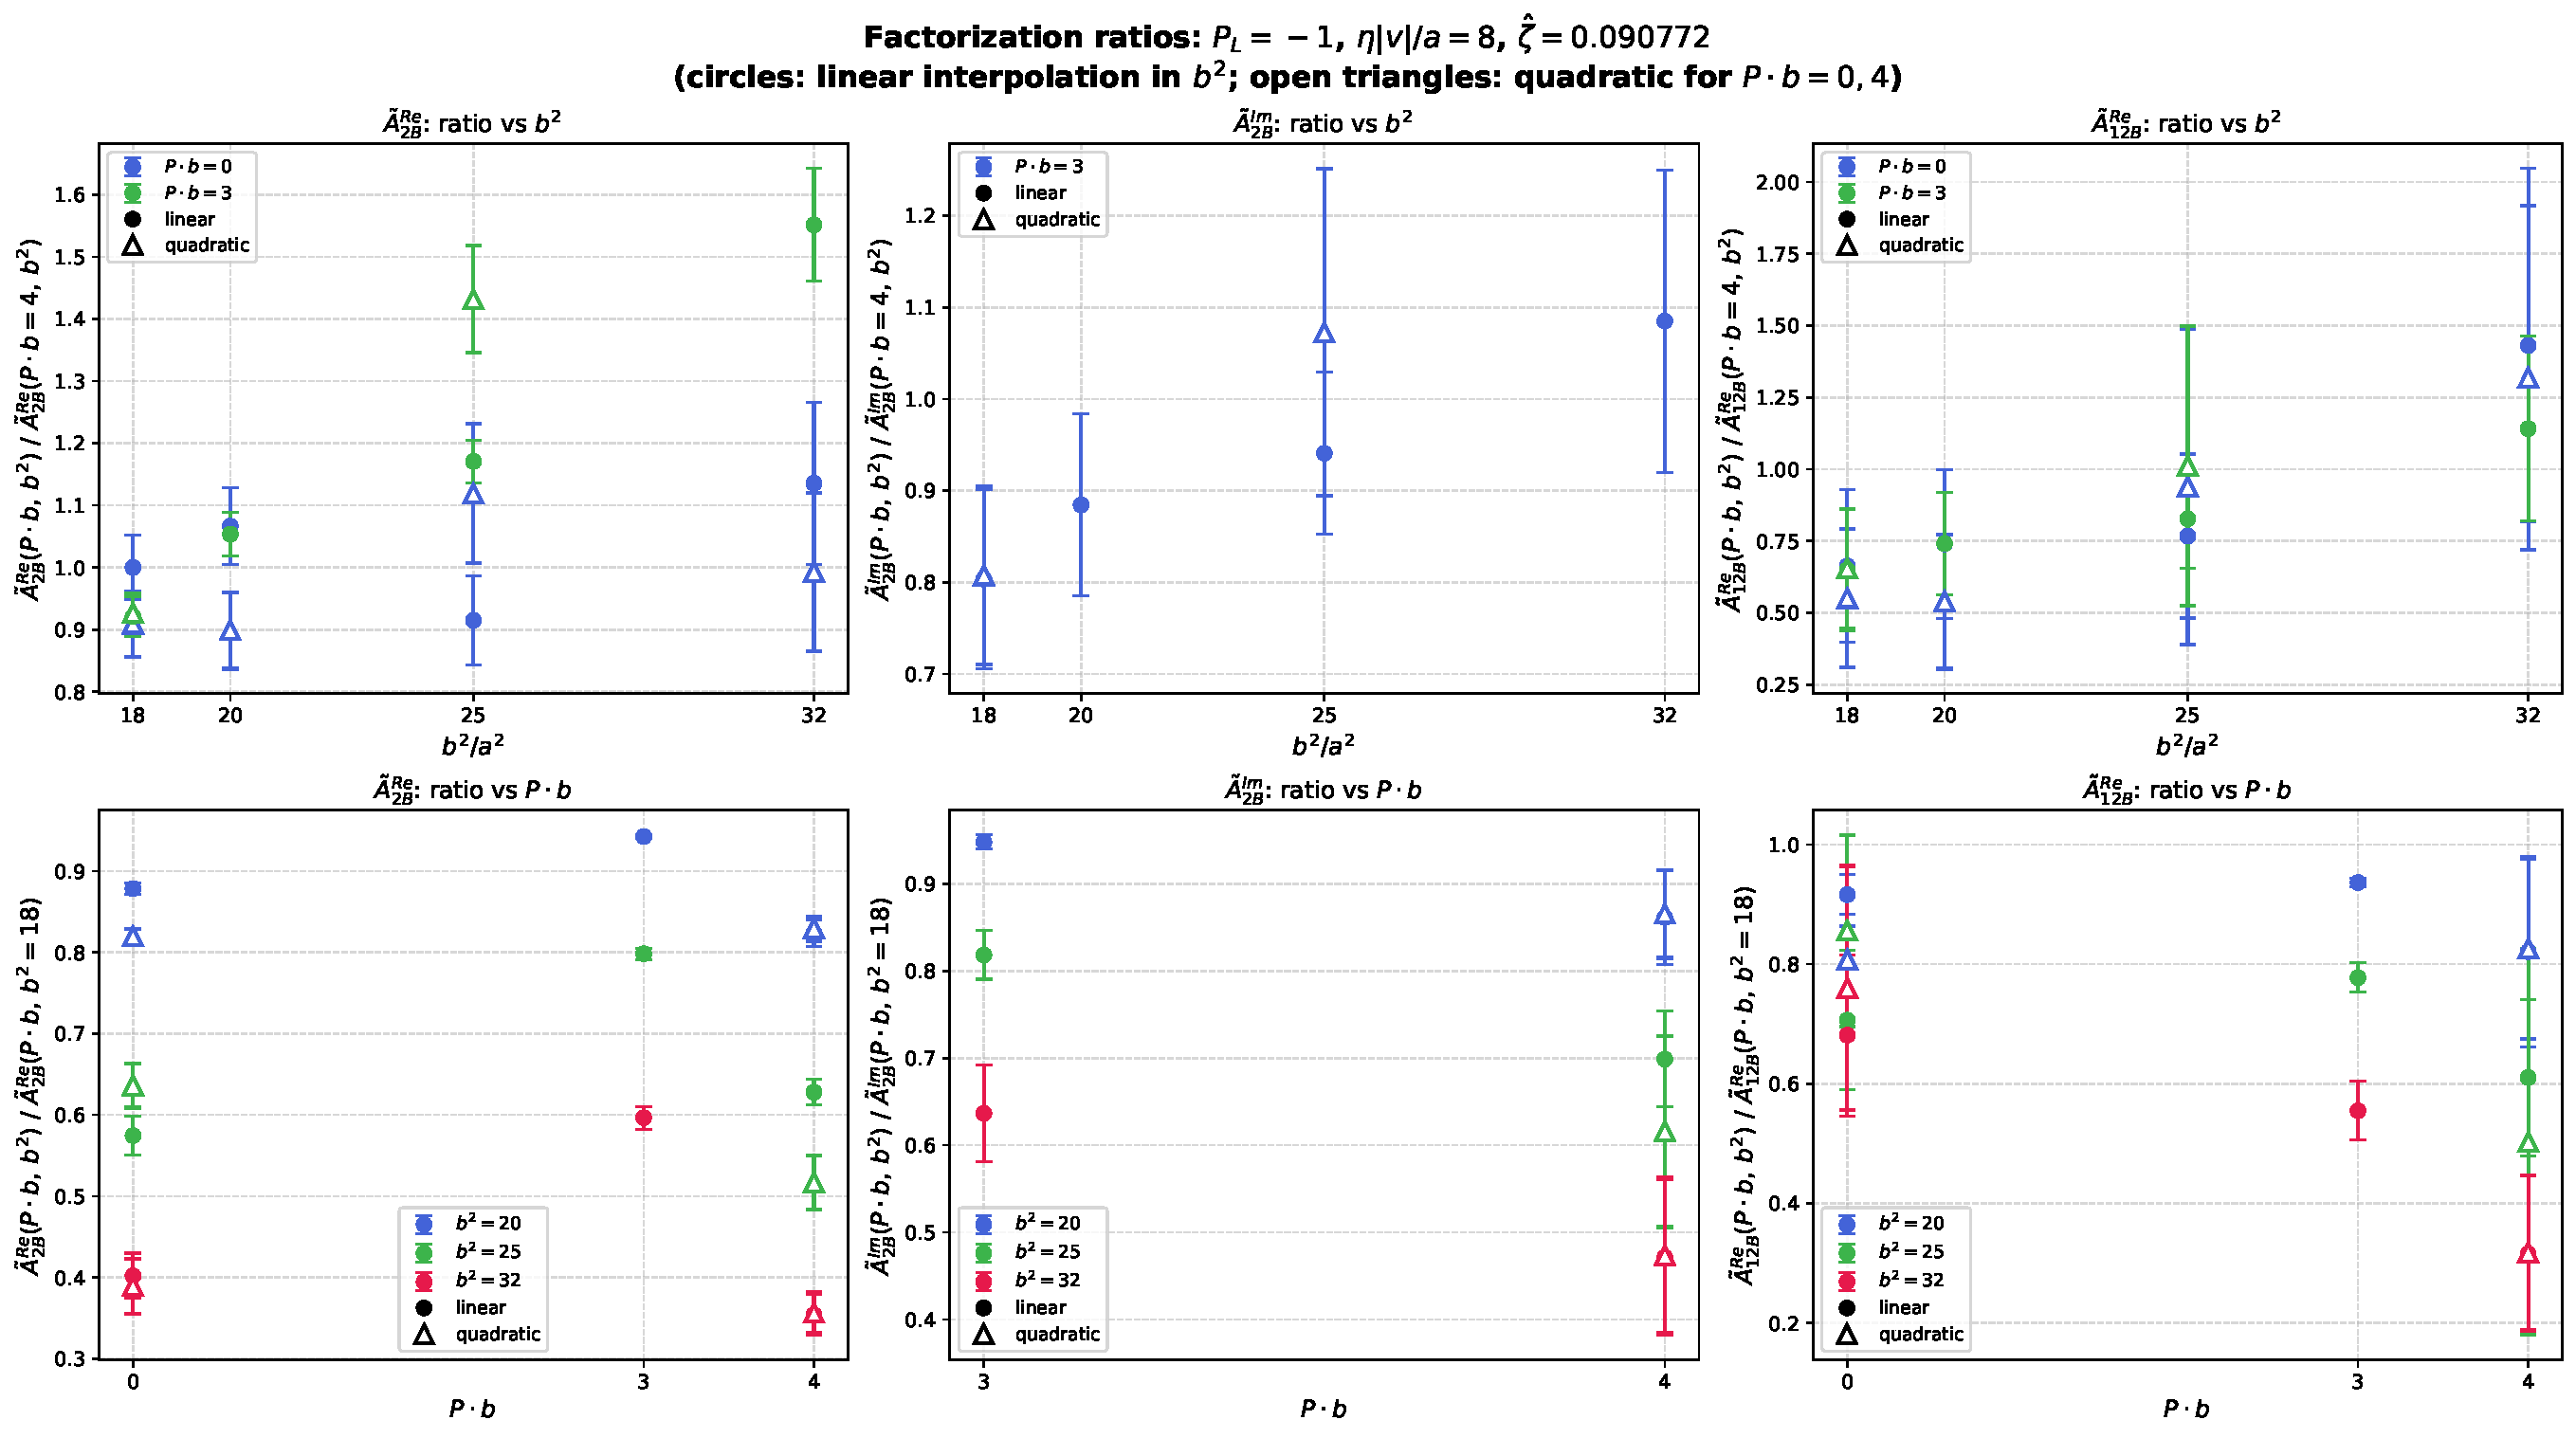
\includegraphics[width=0.8\textwidth]{figures/results/fact_ratio_data.pdf}
\caption{Factorization ratio test on the lattice data at $\eta|v|/a=8$, $P_L=-1$. Top: $T(P\cdot b,b^2)$ against $b^2$. Bottom: $B(P\cdot b,b^2)$ against $P\cdot b$. Under factorization every set of points is flat. Circles: linear interpolation in $b^2$. Triangles: quadratic interpolation on the $P\cdot b=0$ and $4$ rows. Errors are Jackknife errors and do not include the interpolation uncertainty.}
\label{fig:fact_data}
\end{figure*}

\begin{figure}
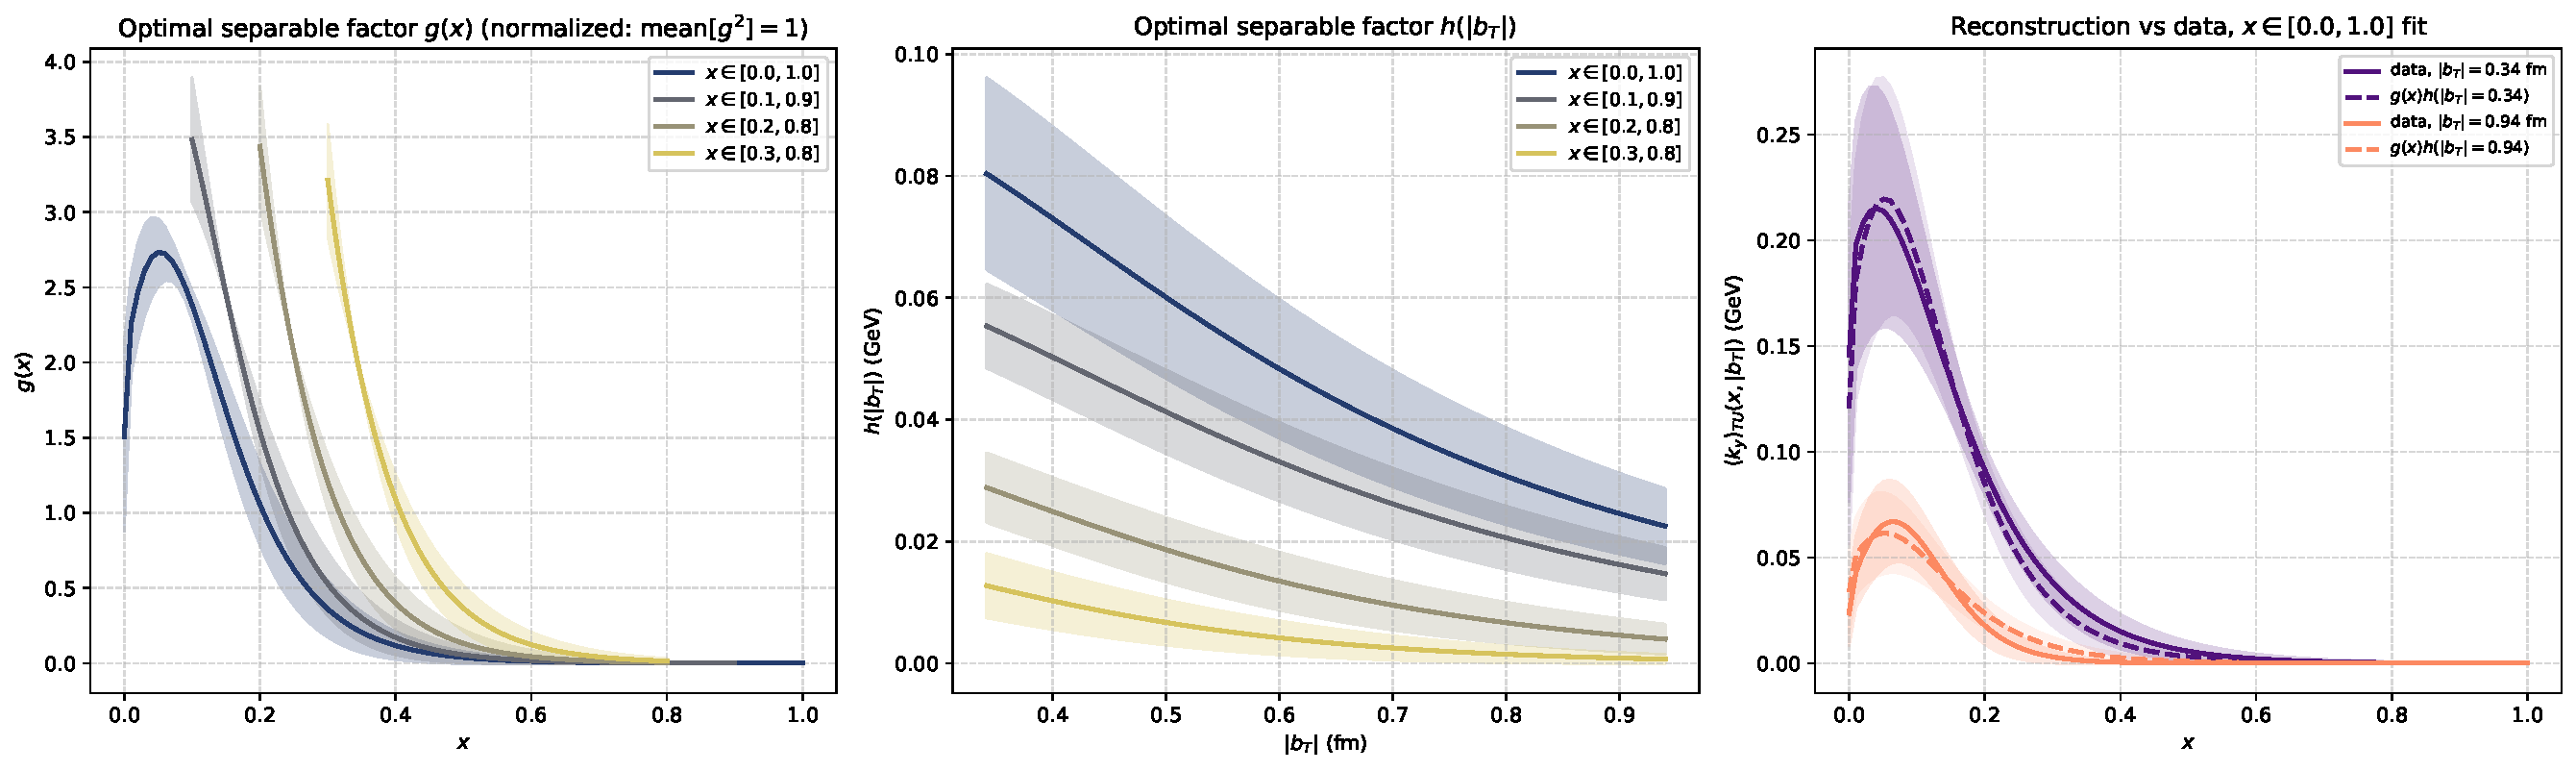
\includegraphics[width=\columnwidth]{figures/results/fact_gh_recon.pdf}
\caption{Optimal separable factors $g(x)$ and $h(|\vect b_T|)$ for the four $x$-windows of Table~\ref{tab:fact_sivers} (left, center) and the reconstruction $g\,h$ (dashed) against the extrapolated Sivers shift (solid) at the smallest and largest $|\vect b_T|$ (right).}
\label{fig:fact_gh}
\end{figure}

\begin{figure}
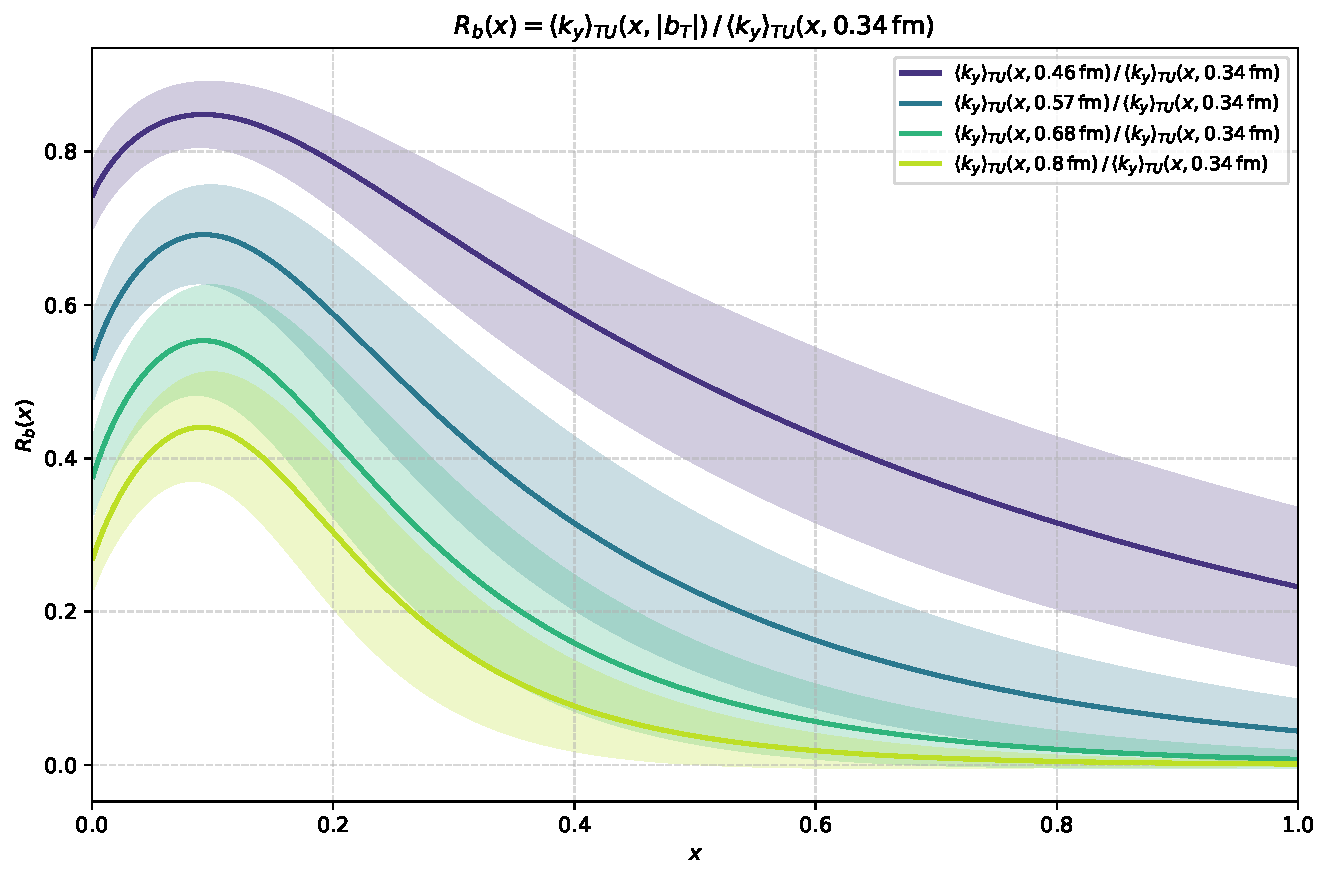
\includegraphics[width=\columnwidth]{figures/results/fact_ratio_x.pdf}
\caption{$R_b(x)$ with $|\vect b_T|_{\rm ref}=0.34$~fm for four values of $|\vect b_T|$. Each curve rises from its $x\to0$ value to a peak near $x\approx0.1$ and then decays instead of staying flat.}
\label{fig:fact_ratio_x}
\end{figure}

\begin{figure}
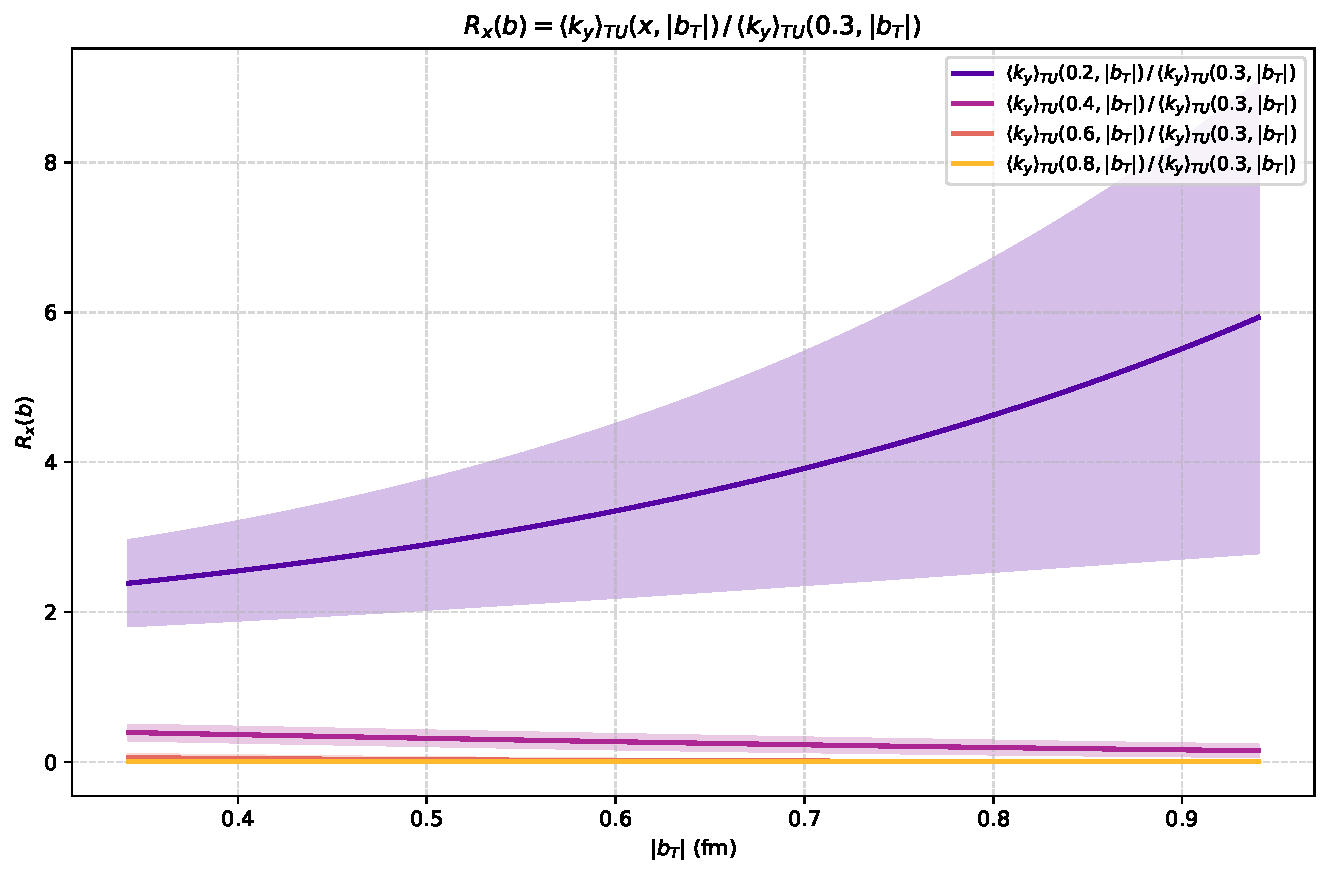
\includegraphics[width=\columnwidth]{figures/results/fact_ratio_bT.pdf}
\caption{$R_x(|\vect b_T|)$ with $x_{\rm ref}=0.3$ for four values of $x$. The $x=0.2$ curve changes by more than a factor of two across the fitted range.}
\label{fig:fact_ratio_bT}
\end{figure}
